\chapter{Junction Current--Voltage Characteristics}
\label{ch:junction-current-voltage}

Bias changes the electrostatic barrier and therefore the minority-carrier
densities at the depletion edges.  Those injected carriers diffuse through the
neutral regions and recombine.  The resulting current is rectifying because a
forward voltage changes the boundary density exponentially, whereas reverse
bias can remove only the equilibrium minority supply.  This chapter develops
the ideal diode equation and its principal recombination and high-injection
corrections \cite[Chap.~3, Sec.~3.4]{szeLee2012}.

\section{Notation and assumptions}

$J$ is conventional current density in $\mathrm{A\,m^{-2}}$.  The subscripts
$n$ and $p$ identify electrons and holes.  $D_n,D_p$ are diffusivities in
$\mathrm{m^2\,s^{-1}}$; $\tau_n,\tau_p$ are minority lifetimes in seconds; and
$L_n=\sqrt{D_n\tau_n}$ and $L_p=\sqrt{D_p\tau_p}$ are diffusion lengths in
meters.  Equilibrium minority densities are
\begin{equation}
 n_{p0}=\frac{n_i^2}{N_A},
 \qquad
 p_{n0}=\frac{n_i^2}{N_D}.
 \label{eq:pn-equilibrium-minority-densities}
\end{equation}

The ideal Shockley treatment assumes an abrupt depletion region, negligible
generation and recombination inside that region, low-level injection,
nondegenerate statistics, constant neutral-region parameters, and negligible
series resistance.

\section{Law of the junction}

A forward voltage $V$ lowers the barrier by $qV$.  Quasi-equilibrium across the
thin depletion region gives the minority concentrations immediately outside it:
\begin{equation}
 \boxed{
 n_p(-x_p)=n_{p0}e^{V/V_T},
 \qquad
 p_n(x_n)=p_{n0}e^{V/V_T}.
 }
 \label{eq:law-of-junction}
\end{equation}
The excess boundary values are therefore
\begin{equation}
 \Delta n_p(-x_p)=n_{p0}(e^{V/V_T}-1),
 \quad
 \Delta p_n(x_n)=p_{n0}(e^{V/V_T}-1).
 \label{eq:pn-boundary-excess}
\end{equation}
This statement is called the law of the junction.  It is a boundary condition,
not a complete transport solution.

\section{Minority diffusion and the ideal diode equation}

In a field-free neutral n-region, steady excess holes satisfy
\begin{equation}
 D_p\frac{\dd^2\Delta p}{\dd x^2}
 -\frac{\Delta p}{\tau_p}=0.
 \label{eq:pn-minority-diffusion}
\end{equation}
For a long base, the physical solution is
$\Delta p=\Delta p(0)e^{-x/L_p}$.  Its junction-edge diffusion current is
$qD_p\Delta p(0)/L_p$.  Adding the symmetric electron contribution gives
\begin{equation}
 \boxed{
 J=J_s(e^{V/V_T}-1),
 \qquad
 J_s=q\left(\frac{D_pp_{n0}}{L_p}
 +\frac{D_nn_{p0}}{L_n}\right).
 }
 \label{eq:ideal-diode-equation}
\end{equation}
$J_s$ is the reverse saturation-current density.  Its strong temperature
dependence arises mainly through $n_i^2$.

For a neutral region of finite length $\ell$, an equilibrium ohmic contact at
$x=\ell$ imposes $\Delta p(\ell)=0$.  The exact profile is
\begin{equation}
 \Delta p(x)=\Delta p(0)
 \frac{\sinh[(\ell-x)/L_p]}{\sinh(\ell/L_p)},
 \label{eq:finite-base-profile}
\end{equation}
and the junction current acquires a factor $\coth(\ell/L_p)$.  The long-base
result follows when $\ell\gg L_p$.

\begin{figure}[htbp]
 \centering
 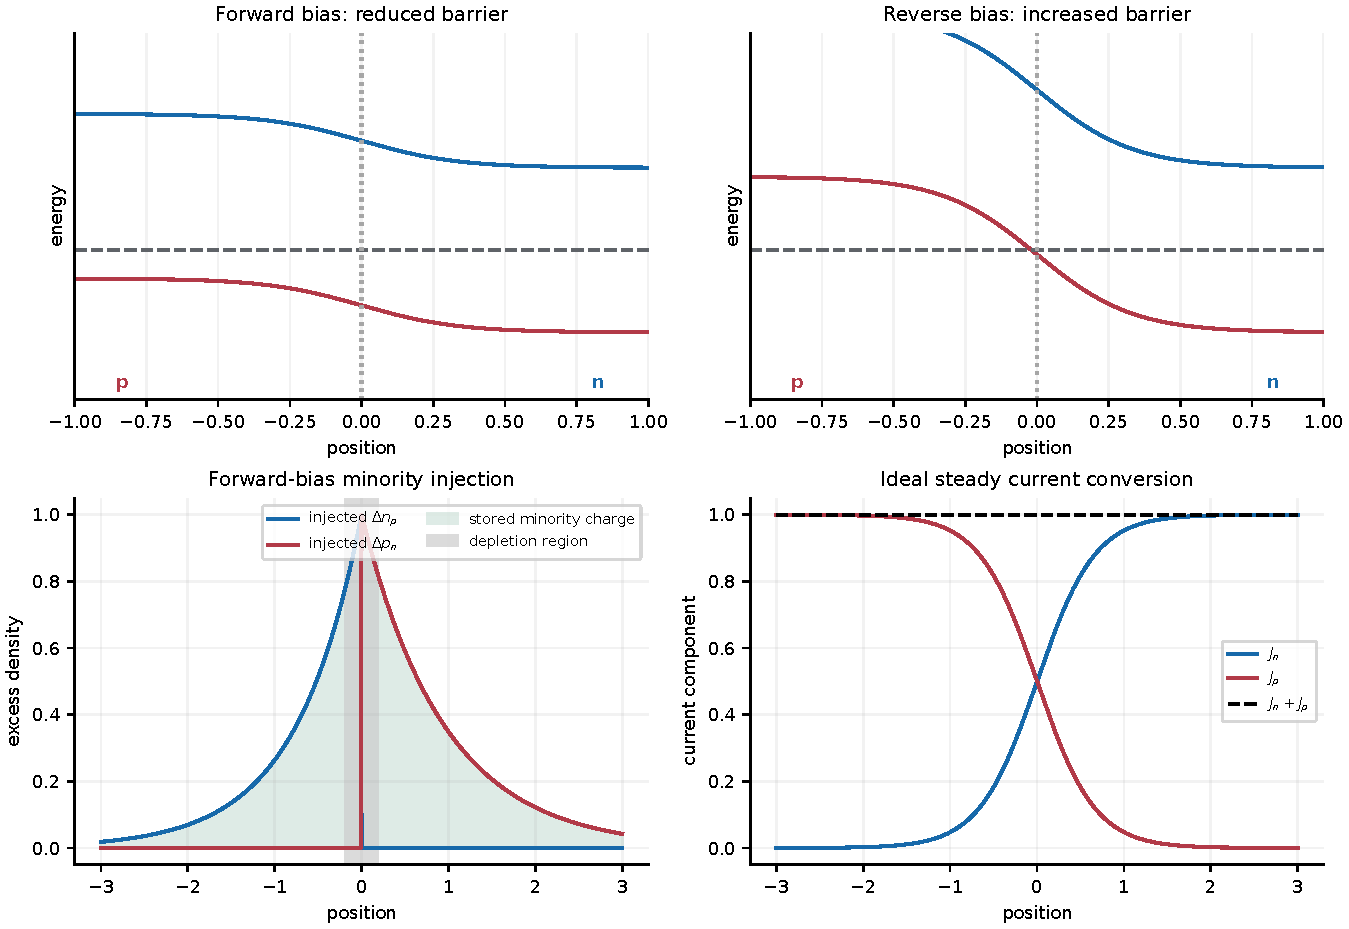
\includegraphics[width=\textwidth]{figures/junction-atlas-injection.pdf}
 \caption{Original forward- and reverse-bias band diagrams, injected
 minority-carrier distributions, stored charge, and conversion between electron
 and hole current components.  These panels cover the subjects of Figs.~14--15
 in Sze--Lee Chapter~3 \cite[Sec.~3.4.1]{szeLee2012}.\figurenotebookmark}
 \label{fig:junction-atlas-injection}
\end{figure}
\figurenotebooktext{figures/18_junction-current-voltage/fig_18_01.ipynb}

\section{Depletion-region generation and recombination}

The ideal model omits centers inside the depletion region.  Under reverse bias,
SRH generation supplies an additional current approximately
\begin{equation}
 J_{\mathrm{gen}}\simeq\frac{qn_iW}{2\tau_g},
 \label{eq:depletion-generation-current}
\end{equation}
for a midgap center and comparable electron and hole generation lifetimes.
Because $W$ grows with reverse bias, this current is not perfectly saturated.

Under forward bias, depletion-region SRH recombination produces approximately
\begin{equation}
 J_{\mathrm{rec}}=J_{02}
 \left(e^{V/(2V_T)}-1\right).
 \label{eq:depletion-recombination-current}
\end{equation}
The exponent corresponds to ideality factor $\eta=2$, while neutral-region
diffusion has $\eta=1$.  A practical exponential model writes
\begin{equation}
 J=J_0\left[e^{V/(\eta V_T)}-1\right],
 \label{eq:diode-ideality-factor}
\end{equation}
where $\eta$ diagnoses a regime but does not identify every microscopic
mechanism uniquely.

\section{High injection and series resistance}

Low-level injection fails when injected minority density approaches the local
majority density.  Charge neutrality then changes the majority concentration,
and the current can approach an $e^{V/(2V_T)}$ dependence even without the same
physics as depletion-region SRH recombination.  Ideality factor alone must
therefore be interpreted with bias and temperature dependence.

At large current, the voltage across neutral material and contacts is no longer
negligible.  If the area-normalized series resistance is $R_s$ in
$\Omega\,\mathrm{m^2}$, the junction voltage is $V-JR_s$ and
\begin{equation}
 J=J_s\left\{\exp\left[\frac{V-JR_s}{\eta V_T}\right]-1\right\}.
 \label{eq:diode-series-resistance}
\end{equation}
This implicit equation bends a semilogarithmic I--V curve away from its ideal
straight line.

\begin{figure}[htbp]
 \centering
 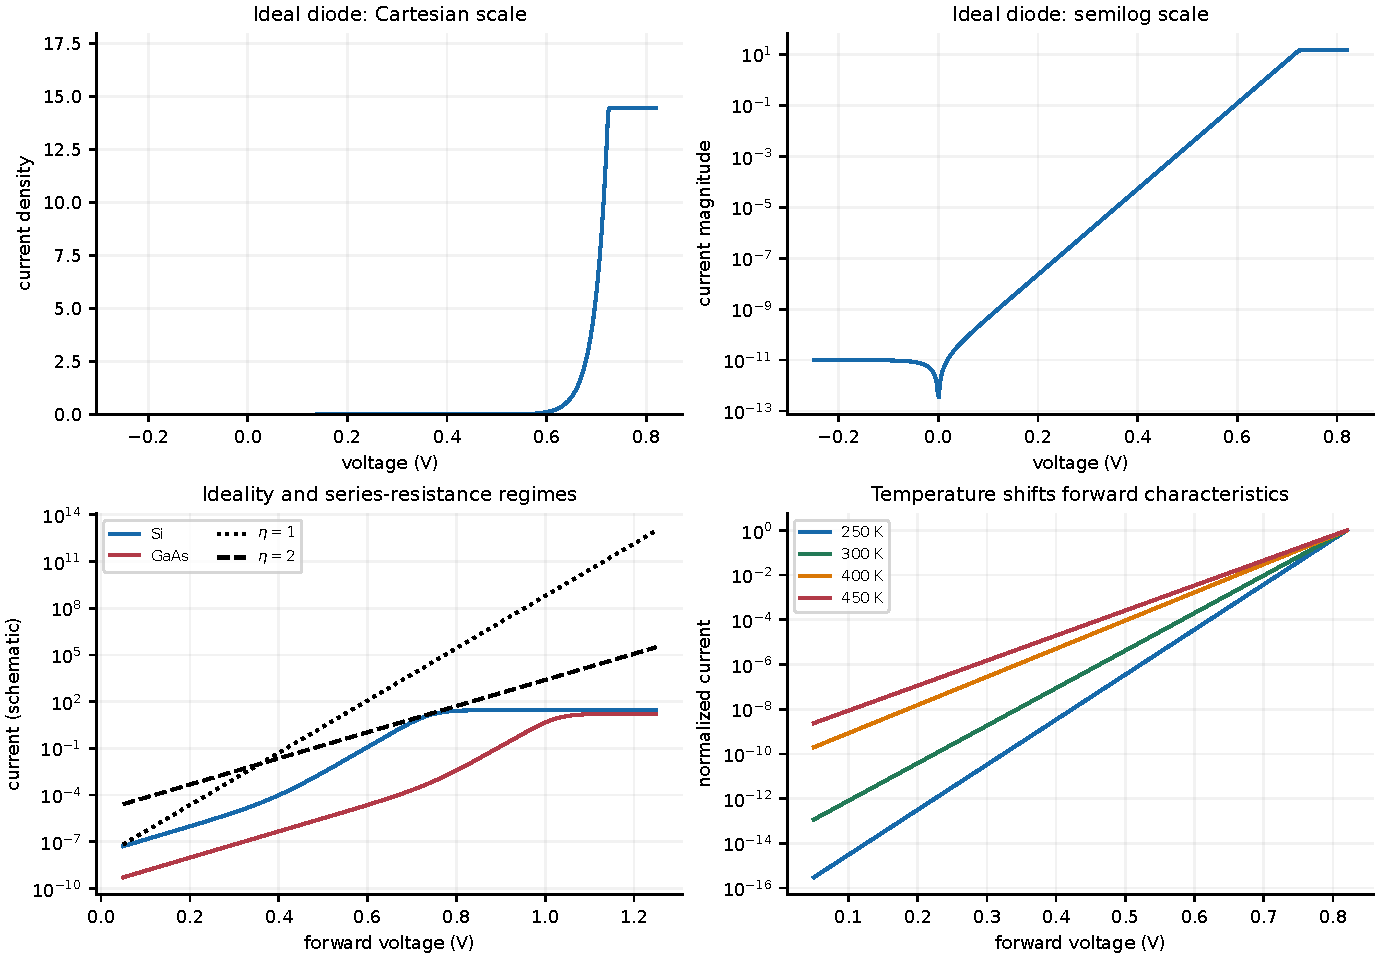
\includegraphics[width=\textwidth]{figures/junction-atlas-diode-characteristics.pdf}
 \caption{Original Cartesian and semilog ideal-diode plots, ideality and
 series-resistance regimes for Si and GaAs, and the temperature shift of a Si
 forward characteristic.  The panels cover the subjects of Figs.~16--17 in
 Sze--Lee Chapter~3 \cite[Secs.~3.4.1--3.4.2]{szeLee2012}.\figurenotebookmark}
 \label{fig:junction-atlas-diode-characteristics}
\end{figure}
\figurenotebooktext{figures/18_junction-current-voltage/fig_18_01.ipynb}

\begin{figure}[htbp]
 \centering
 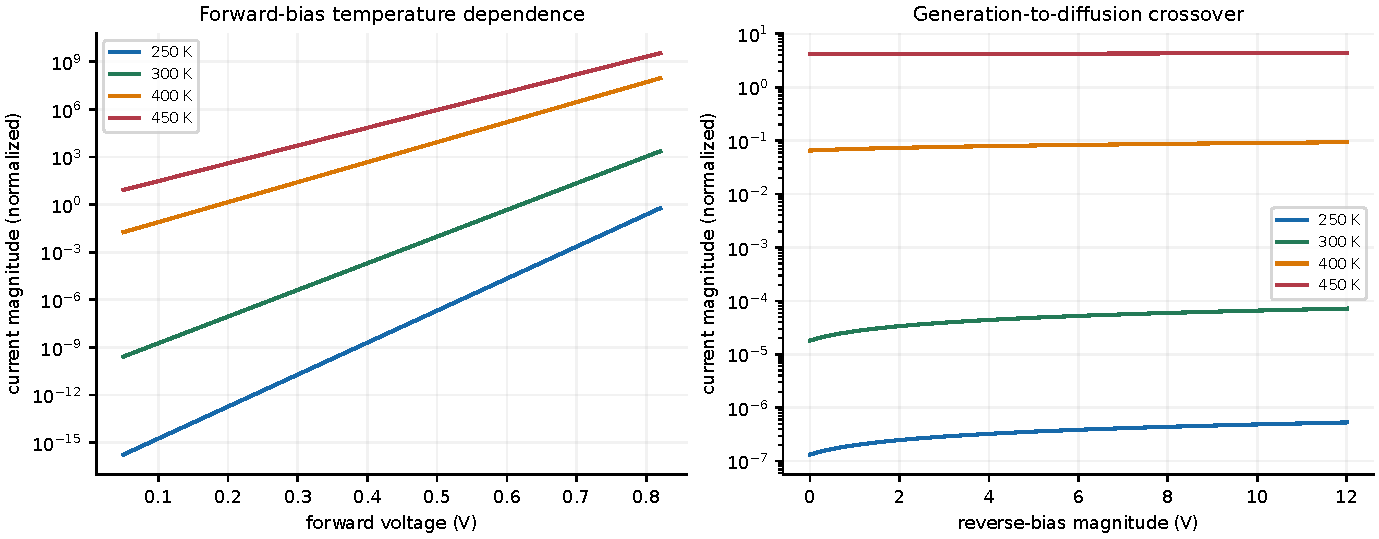
\includegraphics[width=0.94\textwidth]{figures/junction-atlas-temperature-characteristics.pdf}
 \caption{Original forward- and reverse-bias silicon characteristics versus
 temperature.  Reverse current changes from depletion-generation behavior to a
 diffusion-dominated saturation tendency as intrinsic concentration rises.
 These panels cover the physical subject of Fig.~18 in Sze--Lee Chapter~3
 \cite[Sec.~3.4.3]{szeLee2012}.\figurenotebookmark}
 \label{fig:junction-atlas-temperature-characteristics}
\end{figure}
\figurenotebooktext{figures/18_junction-current-voltage/fig_18_01.ipynb}

\section{Finite-difference validation of neutral transport}

On a uniform neutral-region grid, \cref{eq:pn-minority-diffusion} becomes
\begin{equation}
 \Delta p_{i-1}
 -\left(2+\frac{\Delta x^2}{L_p^2}\right)\Delta p_i
 +\Delta p_{i+1}=0.
 \label{eq:minority-diffusion-fd}
\end{equation}
Dirichlet values implement the law of the junction and the equilibrium ohmic
contact.  The edge current is obtained from the discrete gradient.  Comparison
with \cref{eq:finite-base-profile} tests both the profile and the flux, which is
more sensitive to grid resolution.

\begin{figure}[htbp]
 \centering
 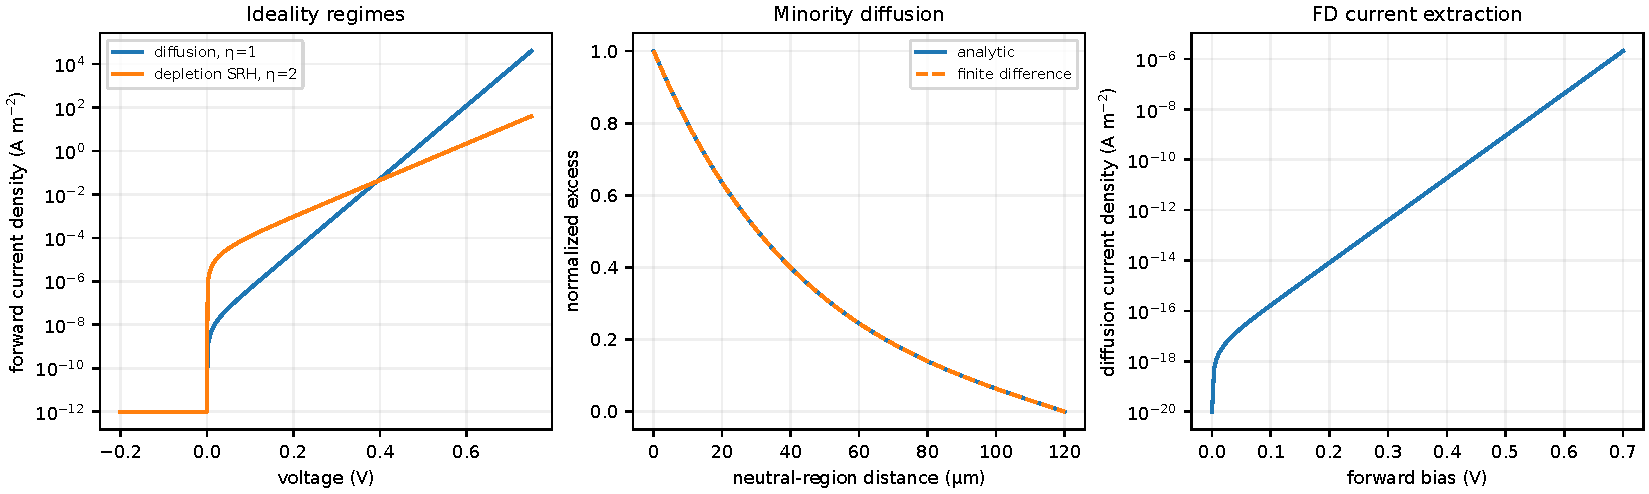
\includegraphics[width=\textwidth]{figures/junction-current-voltage.pdf}
 \caption{Diffusion and depletion-recombination ideality regimes, analytic and
 finite-difference minority profiles, and edge current extracted from the
 numerical gradient.\figurenotebookmark}
 \label{fig:junction-current-voltage}
\end{figure}
\figurenotebooktext{figures/18_junction-current-voltage/fig_18_01.ipynb}

\begin{modelcheck}
For the finite-base problem, the normalized numerical profile converges to
\cref{eq:finite-base-profile}.  The numerical particle flux converges to
$D_p\Delta p(0)\coth(\ell/L_p)/L_p$.  Current vanishes at $V=0$, approaches
$-J_s$ for reverse voltage large compared with $V_T$, and has semilog slope
$\eta V_T\ln 10$ volts per decade in a single exponential regime.
\end{modelcheck}

\begin{boundarybox}
The law of the junction assumes quasi-equilibrium through the depletion layer.
Strong tunneling, large generation, ballistic transport, degeneracy, and
rapidly time-varying bias require a more complete model.  A quantitative device
simulation solves Poisson and both continuity equations self-consistently,
usually with a flux-preserving discretization such as Scharfetter--Gummel.
\end{boundarybox}

\section{Chapter summary}

Bias sets exponential minority-carrier boundary conditions.  Diffusion and
recombination in the neutral regions convert those conditions into the ideal
diode current.  Depletion-region centers introduce generation under reverse
bias and an ideality-two recombination current under forward bias.  High
injection and series resistance produce additional departures.  A finite-
difference minority equation validates the analytic profile and makes explicit
that current is a boundary flux.
